\documentclass{article}
\usepackage{graphicx} % Required for inserting images
\usepackage{float}

\title{Parallel Histogram Equalization}
\author{Skupina 16: Luka Pantar, Mark Loboda}
\date{April 2025}

\begin{document}

\maketitle

\section{Introduction}
\subsection{Serial}
This algorithm performs the \textit{Histogram Equalization} on images on one single thread without any parallelization. Each step of the algorithm is done separately without any optimizations.

\subsection{Parallel}
This algorithm performs the \textit{Histogram Equalization} on images in parallel on the GPU. Steps to transform the image from \textit{RGB} to \textit{YUV} and to compute the histogram are combined, and block size was set to 256, while each pixel is computed by its own thread. Cumulative histogram is done with only one thread, as is the finding of its minimum nonzero value. New luminances lookup table is calculated with one block and 256 threads, one for each different luminance value. Assignment of new pixels and conversion back to RGB is performed in the same step by one thread per pixel in blocks sized 256.

\subsection{Parallel Optimized}
This algorithm optimizes the parallel implementation further with special approaches on steps of the \textit{Parallel Histogram Equalization} algorithm. The histogram is calculated with partial histograms in shared memory, that are combined at the end. Cumulative histogram was implemented according to the document \textit{Parallel Prefix Sum
(Scan) with CUDA} (with avoiding bank conflicts), utilizing 256 threads. Finding the minimum value of cumulative histogram is done with the same number of threads with a parallel reduction algorithm.

\section{Results}
We ran a benchmark of our algorithms by running them nine times for five differently sized images. The first run of each algorithm was discarded, as the execution times were significantly larger because of the caching of kernels on the GPU. Then we also discarded three of the worst times, as the times in some cases are too low to run consistently and sometimes resulted in much higher times, which could've been for other reasons and not the algorithm implementation itself.

The Figure~\ref{fig:avg_times} shows that the execution times for small images stay mostly the same across all implementations. The execution time of the serial implementation quickly falls off when the image size increases, while the parallel algorithms perform much better on all image sizes and lose almost no time with larger images compared to smaller ones. The difference in execution time for larger images is non-significant if we are performing executions for one image at a time. The time difference would, however, become a problem if we used the algorithm to process videos, where we need to process up to sixty images per second.

\begin{table}[H]
    \centering
    \begin{tabular}{| l || c | c | c | c | c |}
        \hline
        Algorithm & 720x480 & 1024x768 & 1920x1200 & 3840x2160 & 7680x4320 \\
        \hline
        Serial & 7.66 & 16.95 & 48.93 & 171.35 & 449.53 \\
        Parallel & 2.69 & 11.71 & 13.72 & 17.89 & 43.49 \\
        Parallel Optimized & 2.46 & 4.26 & 5.95 & 12.34 & 31.66 \\
        \hline
    \end{tabular}
    \caption{Average total time per image for each algorithm measured in \textbf{milliseconds [ms]}.}
    \label{tbl:avg_times}
\end{table}

\begin{figure}[H]
    \centering
    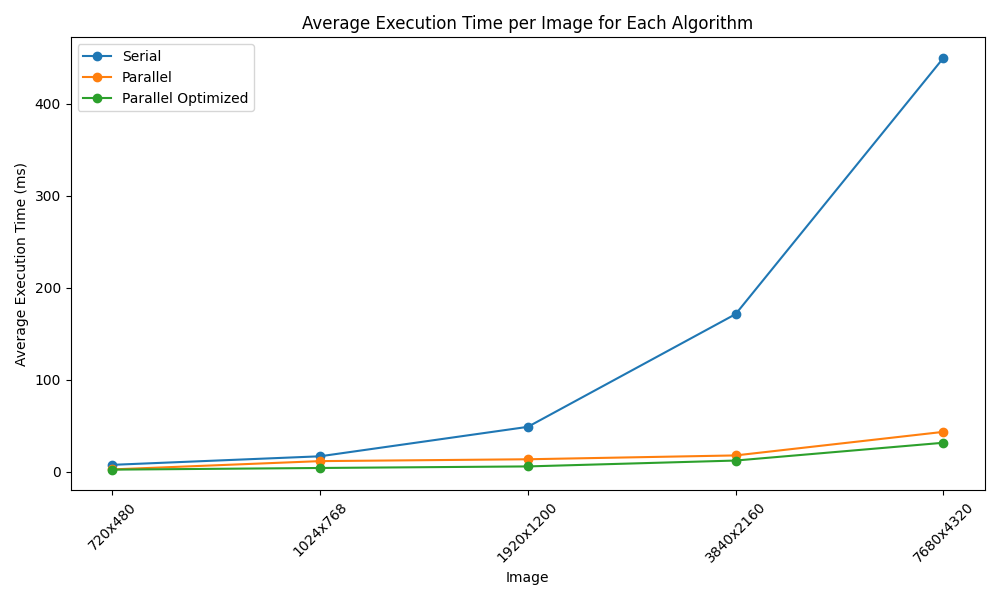
\includegraphics[width=1.0\linewidth]{img/average_times}
    \caption{Average execution time measured in \textbf{milliseconds [ms]} of each algorithm for each image, shown in Table~\ref{tbl:avg_times}.}
    \label{fig:avg_times}
\end{figure}

Figure~\ref{fig:speedups} and Table~\ref{tbl:speedups} show the speedups calculated between given algorithms. The speedup is calculated by dividing the average times of execution of both algorithms. We can see that the parallel algorithms benefit greatly with larger images, as the speedup increases significantly when compared to the serial. We found it interesting as well that the optimized parallel algorithm benefited the most on images of medium size but fell off a bit for larger and smaller images.

\begin{table}[H]
    \centering
    \begin{tabular}{| l || c | c | c | c | c |}
        \hline
        Comparison & 720x480 & 1024x768 & 1920x1200 & 3840x2160 & 7680x4320 \\
        \hline
        Parallel/Serial & 2.85 & 1.45 & 3.57 & 9.58 & 10.34 \\
        Parallel Optimized/Serial & 3.12 & 3.98 & 8.22 & 13.89 & 14.20 \\
        Parallel Optimized/Parallel & 1.09 & 2.75 & 2.31 & 1.45 & 1.37 \\
        \hline
    \end{tabular}
    \caption{Average speedup calculated between execution times for each image.}
    \label{tbl:speedups}
\end{table}

\begin{figure}[H]
    \centering
    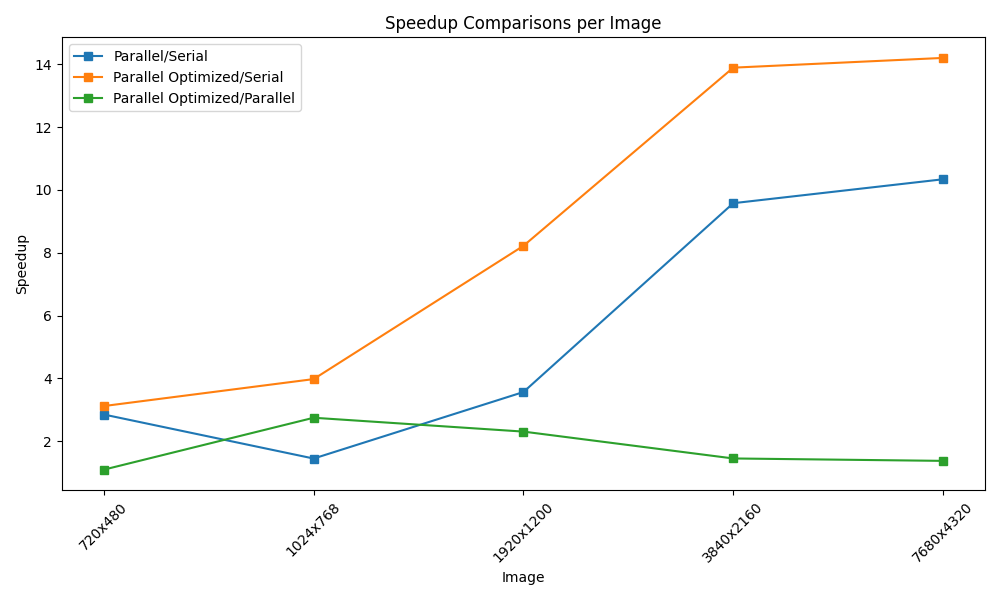
\includegraphics[width=1.0\linewidth]{img/speedup_comparisons}
    \caption{Average speedup calculated between execution times for each image, shown in Table~\ref{tbl:speedups}.}
    \label{fig:speedups}
\end{figure}

Overall speedup on images can mostly be attributed to parallelization of histogram calculation (up to 60 times speedup) and assignment of new pixel values (up to 190 times speedup). As for the further optimizations done to parallel algorithm, the biggest impact had the use of shared memory - providing up to 4 times speedup. Parallel scan and finding of minimum value only yielded at most 20\% improvement. 

\end{document}
